\documentclass[preprint,12pt]{elsarticle} 

\usepackage{slashed}
\usepackage{graphicx}
\usepackage{amssymb}
\usepackage{mathtools}
\usepackage{bbold}
\usepackage{amssymb,latexsym}
\usepackage{amsmath,amsbsy,bbm}
\usepackage{multirow}
\usepackage[vcentermath]{youngtab}
\usepackage{nicefrac}
\usepackage[perpage]{footmisc}
\usepackage{wrapfig,lipsum,booktabs}


\usepackage{caption}
\usepackage{subcaption}
\usepackage{graphicx}
%\usepackage{physics}
\usepackage{floatrow}
%\newfloatcommand{capbtabbox}{table}[][\FBwidth]
\newfloatcommand{capbtabbox}{table}[][0.45\textwidth]

\DefineFNsymbols*{lamportnostar}[math]{\dagger\ddagger\S\P\|{\dagger\dagger}{\ddagger\ddagger}}
\setfnsymbol{lamportnostar}
\renewcommand\thefootnote{\fnsymbol{footnote}}

\usepackage[dvipsnames]{xcolor} 
\newcommand{\es}{1\text{\scriptsize s}}
\newcommand{\zs}{2\text{\scriptsize s}}
\newcommand*{\mprime}{^{\prime}\mkern-1.2mu}
\newcommand{\largescale}{\ensuremath{\Lambda_\text{Hi}}}
\newcommand{\lc}{\ensuremath{\lambda_c}}
\newcommand{\fm}{\ensuremath{\,\text{fm}^{-1}}}
\newcommand{\abb}{\ensuremath{2\!+\!1^{(A-1)}}}
\newcommand{\red}[1]{\textcolor{red}{#1}} 
\newcommand{\green}[1]{\textcolor{green}{#1}} 
\newcommand{\blue}[1]{\textcolor{blue}{#1}} 
\newcommand{\lec}{C^\Lambda}
\newcommand{\led}{D^\Lambda}

\newcommand{\ddrei}[1]{\delta_{\tiny \Lambda}^{(3)}\!\big(#1\big)}
\newcommand{\wrt}{\textit{wrt.}~}
\newcommand{\etc}{\textit{etc.}~}
\newcommand{\eg}{\textit{e.g.}~}
\newcommand{\ie}{\textit{i.e.}~}
\newcommand{\eftnopi}{\mbox{EFT$(\not \! \pi)$}}
\newcommand{\ve}[1]{\ensuremath{\boldsymbol{#1}}}
\newcommand{\rms}[1]{\ensuremath{\langle r(#1)\rangle}}
\newcommand{\ls}{\ve{L}\cdot\ve{S}}
\newcommand{\be}{\begin{equation}}
\newcommand{\ee}{\end{equation}}
\newcommand{\bra}{\big\langle}
\newcommand{\ket}{\big\rangle}
\newcommand{\hl}{\big\vert}
\newcommand{\vcl}[1]{\ensuremath{\bar{\boldsymbol{r}}_\text{\tiny #1}}}
\newcommand{\vsp}[1]{\ensuremath{\boldsymbol{r}}_\text{\tiny #1}}
\newcommand{\la}{\label}
\newcommand{\figref}[1]{fig.~\ref{#1}}
\newcommand{\tabref}[1]{table~\ref{#1}}

\begin{document}

\title{Multi-fermion systems with contact theories}
\author{M.~Sch{\"a}fer}\address{Czech Technical University in Prague, Faculty of Nuclear Sciences 
and Physical Engineering, B\v{r}ehov\'{a} 7, 11519 Prague 1, Czech Republic} 
\author{L.~Contessi} 
\address{Racah Institute of Physics, The Hebrew university, 91904 Jerusalem, 
Israel} 
\address{ESNT, IRFU, CEA, Universite Paris Saclay, F-91191 Gif-sur-Yvette, France} 
\author{J. Kirscher}
\address{Theoretical Physics Division, School of Physics and Astronomy,
The University of Manchester, Manchester, M13 9PL, United Kingdom} 
\date{October 2018}


\begin{abstract}
The particle-stability of isomassive fermionic systems is analysed
for constituent numbers which exceed the number of accessible flavour states. The interaction is taken as an 
effective field theory of momentum- and flavour-independent two- and three-body
regulated contact terms which are renormalized to shallowly bound dimer and trimer states.
The regulator dependence of the stability of these systems is assessed as a function of
particle number and the proximity of the interaction to two-body unitarity.
% which is parametrized by an increasing ratio between trimer and dimer binding energy.

We find no system of mixed-spatial symmetry stable with respect to
a decay into fragments with spatially symmetric wave functions if the range of the
interaction is shorter than a number- and renormalization-condition-dependent
critical range.
We elaborate on the consequences of our results for the systematic description of
atomic and nuclear systems. For the latter, in particular, the study provides
strong evidence for an inclusion of momentum-dependent interaction terms in order
to describe $P$-wave stable systems such as $^6$Li and $^8$Be effectively.
\end{abstract}

\maketitle

\section{Introduction -- Shelley}

What properties of an $A$-body system are dynamical consequences of a resonant two-body interaction
with its discrete three-body scale invariance broken by a single bound trimer?
Such constructive correlations between the two- and three-body parameters and larger systems have been
identified for particles obeying Bose statistics, equivalently, for a number of fermions equal or less
than the dimension of their flavour space. Prominent examples include
the linear dependence of the four-boson ground-state energy on the trimer energy (Tjon line~\cite{tjon}), and
the more recent discovery~\cite{von_Stecher_2010} of a sequence of universal pairs of $A$-body states
each below the $A-1$ normal threshold terminating with an Efimov trimer.

The aim of this work is to study such correlations between microscopic and macroscopic observables for systems comprised of
a number of particles exceeding the dimension of an internal flavour space.
The demand of an antisymmetric total wave function thus implies
a spatial state of mixed symmetry\footnote{We refer to a system of $A$ $N$-flavour fermions with $A>N$
as $N^a \oplus b$ with $a$ $N$-uplets of fermions which can share the same spatial quantum states, and $b<N$ are the residual
particles which are not enough to fill the flavour degeneracy of the states.
This notation has the advantage to immediately expose immediatly the number of particles not on-shell for the Pauli interaction.
E.g. in this notation the nuclear $^6$Li is noted as $4 \oplus 2$; A hypothetical system of 33 atomos of Helium-3 (fermions with spin $1/2$) are noted as $2^{16} \oplus 1$;}.
%we generalize the notation (\eg~see Ref.~\cite{PhysRevA.92.053624}) of a $p+q$ fermionic problem in which $p$ identical fermions interact with another set of $q$ identical fermions such that $\underbrace{1+\ldots+1}_{\text{$A$ terms}=:1^A}$ denote the $A$-different-fermion system \footnote{which in this study, that employ a flavour independent interaction, is also noted as bosonic-like system due to the corrispondence of the spatial part of the groundstete in the two cases} 
%$2+1^3$ being two spin-up and one spin-down neutron(s), and two protons, one spin-up and one spin-down, \ie, 5-helium, \etc. 

To study the essence of the problem, we commence by considering the stability of systems with only one fermion more than flavour states accessible.
This model system comprises $A\oplus1$ equal-mass particles, two of which are forced into the same flavour state.
For this investigation it has been chosen to employ contact effective field theory as it is the simplest effective theory which can grasp non trivial phenomena in many-particle physics.
To minimize the amount of mass-scales present in the theory we focus the study of systems which are close to the unitary limit (which comprises the nuclear case [Kievski]), where the dimer resides on or close to the two-body threshold and shows exact or approximate scale invariance proprieties.
Under these conditions a three-body Efimov spectrum accumulates at the same threshold, replacing the continuum scale invariance with a discrete one.

This theory has been used to study the proprieties of 2[2bosons], 3[3bosons], and many\cite{manybosons} bosons at unitarity; and of four-nucleon system \cite{Barnea:2013uqa} predicting the presence of spatially symmetric groundstates and a consistent binding of $^4$He nucleus.
Studies which extended to fermioninc systems with multiple paricle of the same specie showed that in the case of three\cite{Kartavtsev_2007} and four\cite{petrov_dimerov, Petrov:2005zz,PhysRevA.92.053624} isomassive two-flavour fermions no stable states are present.
In the nuclear sector a similar extension has been done for $^{6}$He\cite{Gattobigio:2019omi}
\footnote{M. Gattobigio et al. do not employ a renormalized contact EFT, but a short range theory close to universality which correspond to a Contact EFT interaction with relatively large cut-off.}
and $^{16}$O\cite{Contessi:2017rww}.
This two nuclei appear to be unstable against the decay in spatially symmetric fragments (I.e. alpha particles) in those two studies.
It is still unclear \red{and we want to discover} if the impossibility to stabilize such systems is a universal behaviour.
However, there are no doubts that the description of those states is a fundamental requirement for nuclear systems since they are close to universality and present bound states for systems with more than four nucleons.

To investigate universality beyond spatially simmetric bound-states, we begin with a description of the employed interaction theory in terms of its Hamiltonian, regularization, and renormalization. 
Then, results on the regulator dependence of the stability of $A\oplus 1$ and $A\oplus 2$ as they follow from this theory are presented.
The nuclear systems 6-lithium and 8-beryllium are treated separately.
Based on the results, we comment on potential consequences for the nuclear contact EFT.
%In an appendix, we present the structure and a succinct guide to an effective two-fragment interaction which allows for the description of larger systems.

%%%%stuff for theory framework
%For simplicity all the calculations have been made with fermions of mass $938.858$ MeV, corresponding to the averaged nucleonic mass.
%However, the results remain general since the energy scales of the systems can be rescaled in the concept of system universality.


%Thus, the problem is specified through five parameters, the particle's mass ($m$), the number $A$, a dimer and trimer
%binding energy which calibrate the two interactions strengths, and a regulator scale which represents a particular
%short-distance behaviour \wrt which the dimer and trimer are invariant by definition.
\newpage
\section{Introduction -- Byron}
The entirety of observables on an $A$-body system can be split into two classes. In one, there are those
which can be parametrized with certain properties of subsystems ($A_\text{sub}<A$) by solving the same
dynamical equation for the respective number of particles. In the other class, one finds all observables
characteristic to the interaction of $A$ particles which cannot be related to a ``few'' parameters of the
subsystems. A systematic way to assign a given observable to either of these classes is to our best knowledge unknown.

However, progress has been made to categorize particular nuclear and atomic quantities. Employing the
effective-field-theory (EFT) formalism, it has been shown~\cite{Bedaque:1998kg}, for instance, that the binding energy 
of three bosons (trimer)
is unrelated to two-body data if the latter sustains a bound state with spatial correlations significantly larger
than the two-particle interaction which generates it (unitary system). The (linear-in-a-finite-interval) dependence
of the ground-state
energy of the four-boson system on the three-boson energy (Tjon line), in contrast, was identified as a
universal consequence of this two-body unitarity~\cite{Platter:2004zs}.
For bosonic atoms, a generalization of this correlation has been
established numerically (see Ref.\cite{von_Stecher_2010} for the first step)
by identifying a pair of one deep and one shallow $A+1$ boson state attached to
a universal $A$-boson state starting with a fixed trimer.
Thereby, a non-trivial property of $A$ particles can
be predicted solely with two- and three-body data.

It is the aim of this work, to assess the dependence of such a correlation between macroscopic and microscopic
dynamics on any deviation from the purely bosonic character of the particles.
The latter allows all particles to occupy the same spatial state which they cannot if the system comprises
more elements than internal flavours\footnote{We generalize the notation (see \eg~Ref.~\cite{PhysRevA.92.053624})
of a $p+q$ fermionic 
problem in which $p$ identical fermions
interact with another set of $q$ identical fermions such that $\underbrace{1+\ldots+1}_{\text{$A$ terms}=:1^A}$ is 
the $A$-boson problem, $2+1^3$ being two spin-up and one spin-down neutron(s), and two protons, one spin-up and
one spin-down, \ie, 5-helium, \etc}.
To study the essence of the problem, we commence by considering the stability of systems with only one particle
more than flavour states accessible as they depend on the short-distance structure of the same two- and three-body
interaction which is known to universally create such stable states below a threshold corresponding to the separation
of one particle. This model system comprises $A+1$ equal-mass particles, two of which are forced into the same
flavour, \ie, spin-isospin, state whose dynamics are dictated by an $A+1$-body Schr\"odinger equation which
represents the leading order of an effective field theory as pertinent to a bosonic system.
Thus, the problem is specified through five parameters, the particle's mass ($m$), the number $A$, a dimer and trimer
binding energy which calibrate the two interactions strengths, and a regulator scale which represents a particular
short-distance behaviour \wrt which the dimer and trimer are invariant by definition.

We focus the study on systems which are close to the so-called unitary limit where the dimer resides on or close to
the two-body threshold under conditions which a three-body Efimov spectrum accumulates at the same threshold.
Besides numerous atomic systems which exhibit such spectra in appropriately tuned traps,
we address nuclei, in particular. The latter are amenable to a description with neutrons and protons and
therefore do allow for a totally spatial symmetric state only up to $A=4$ (ground state of the $\alpha$ particle).
The generic stability problem states above translates into that of the short-distance/renormalization-group
invariance of the resonant 5-helium, and the 6-lithium and 8-beryllium stable ground states. 

We begin with a description of the employed interaction theory in terms of its 
Hamiltonian, regularization, and renormalization. 
Then, results on the regulator dependence of the stability of $P$-wave systems with up to $A>120$ as they follow
from this theory are presented.
The nuclear systems 6-lithium and 8-beryllium are treated separately.
Based on the results, we comment on potential consequences for the nuclear contact EFT.
In an appendix, we present the structure and a succinct guide to an effective two-fragment interaction which
allows for the description of larger systems.

\section{Theoretical framework -- Shelley}

A minimal theory (see \eg~Refs.\cite{Lepage:1997cs,vanKolck:1999mw, Bedaque:1998kg, Braaten:2004rn, Hammer:2017tjm, 
Hammer:2019poc}) of non-relativistic point particles exhibiting two- and three-body correlations which extend
well beyond the support of their mutual interaction, which can be systematically refined to attain a desired accuracy,
which can be related to an underlying theory resolving substructure,
and which is itself a fundamental theory for effective halo and cluster models
is represented by: a Hamiltonian comprising a zero-range two- and three-body
vertex

\begin{equation}
H = - \sum_i \frac{\hbar^2}{2m}\ve{\nabla}^2+ \lec \sum_{i<j}{\delta_\Lambda(\ve{r}_i-\ve{r}_j)} 
+ \led \sum_{ i<j<k \atop \text{cyc} }\delta_\Lambda(\ve{r}_i-\ve{r}_j)\delta_\Lambda(\ve{r}_i-\ve{r}_k);
\label{eq:hamiltonian}
\end{equation}

an expansion of the ensuing amplitude whose leading order(LO) is represented by all Born terms
depending solely on the coupling constants $\lec$ and $\led$, while parameters representing the aforementioned
refinements enter perturbatively at the order given na\"ively by their higher mass dimension;
the renormalization of unobservable behaviour of the interaction for momenta above a characteristic scale
which is reflected in the singular zero-range potential.

Specific to this work is the Gaussian regulator 
\mbox{$\delta_\Lambda(\ve{x}) \propto\Lambda^3 e^{-\frac{\Lambda^2}{4}\ve{x}^2}$}
which introduces a cutoff parameter $\Lambda$.
The unobservable $\Lambda$ dependence of $\lec$ and $\led$ was chosen to render
the energy of a single bound state in each, the two- and three-body system, respectively, $\Lambda$-independent.
Whether or not the induced dependence of another amplitude on the particular choice for $B(2)$ and $B(3)$
converges for $\Lambda\to\infty$, classifies it as either universal or emergent in the sense alluded to in the introduction.
By using the average nucleon mass $m=938~$MeV,
$B(2)=1$~MeV with $B(3)\in\lbrace1.5,\,3,\,4\rbrace$~MeV, and $B(2)=0^+$~MeV with $B(3)=3$~MeV, we
consider a class of few-body systems with \abb~statistics as they 
approach the unitary limit via increasing the numerator instead of the denominator of the
ratio $B(3)/B(2):=\Lambda^*$.

The pionless, nuclear EFT is renormalized separately to yield the deuteron and triton binding energies of $B(2)=2.22$~MeV
and $B(3)=8.48$~MeV, respectively. 
Technically, the necessary fits employ precise SVM and RGM variational diagonalization methods for $\led$,
while $\lec$ was determined via a Numerov-type integration of the appropriate one-dimensional radial
Schr\"odinger equation.

\section{Results}

We discuss results of the theory for $A$-body systems with at least $A$ fermionic
flavours, \ie, those with a bosonic ground state, before considering systems
which contain one and two interacting particles more than accessible flavours.
For each system, we analyse its dependence on the interaction-range-characterizing
regulator parameter ($\Lambda$), the proximity of the theory to two-body unitarity, which we parametrize with the ratio between dimer and trimer binding energies
($B(3)/B(2):=\Lambda^*$), and we study the spatial symmetry of the ground states.
Finally, the many-body limit $A\gg1$ is investigated.

\begin{figure}
    \centering
    \begin{subfigure}[t]{0.45\textwidth}
        \centering
        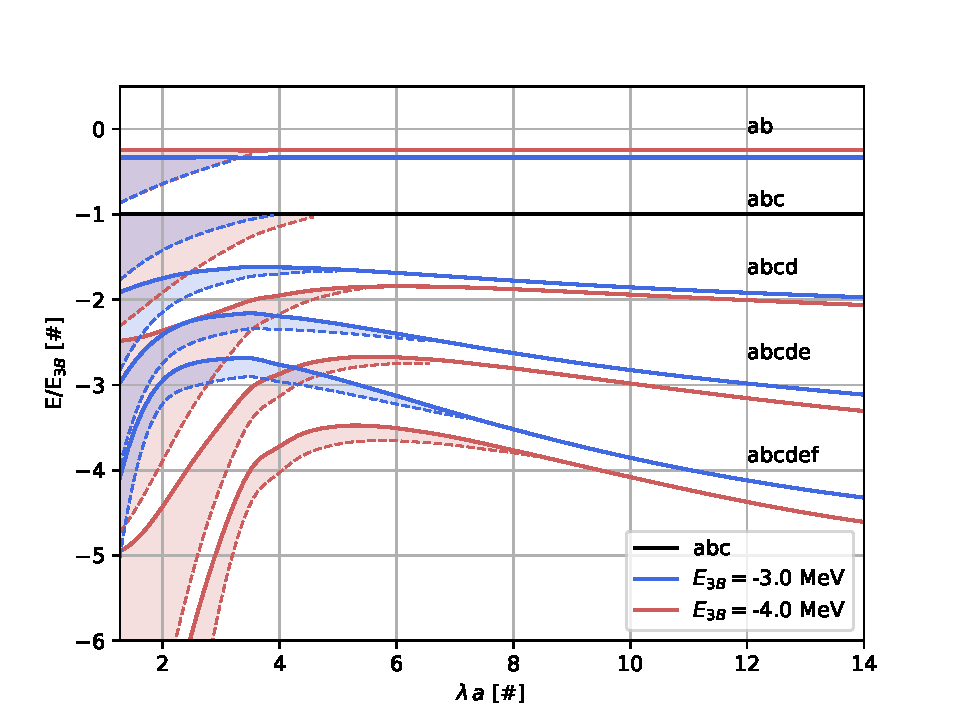
\includegraphics[width=\linewidth]{./p-systems-vs-l} 
        \caption{(Colors online) Cutoff dependence of ground-state energies of $A$-boson (solid line) and \abb
        (dashed line) systems for two trimer binding energies, $B(3)=3~$MeV (blue) and $B(3)=4~$MeV (red), and
        a single dimer constraint to $B(2)=1~$MeV.}
        \label{fig:threshold}
    \end{subfigure}
    \hfill
    \begin{subfigure}[t]{0.45\textwidth}
        \centering
        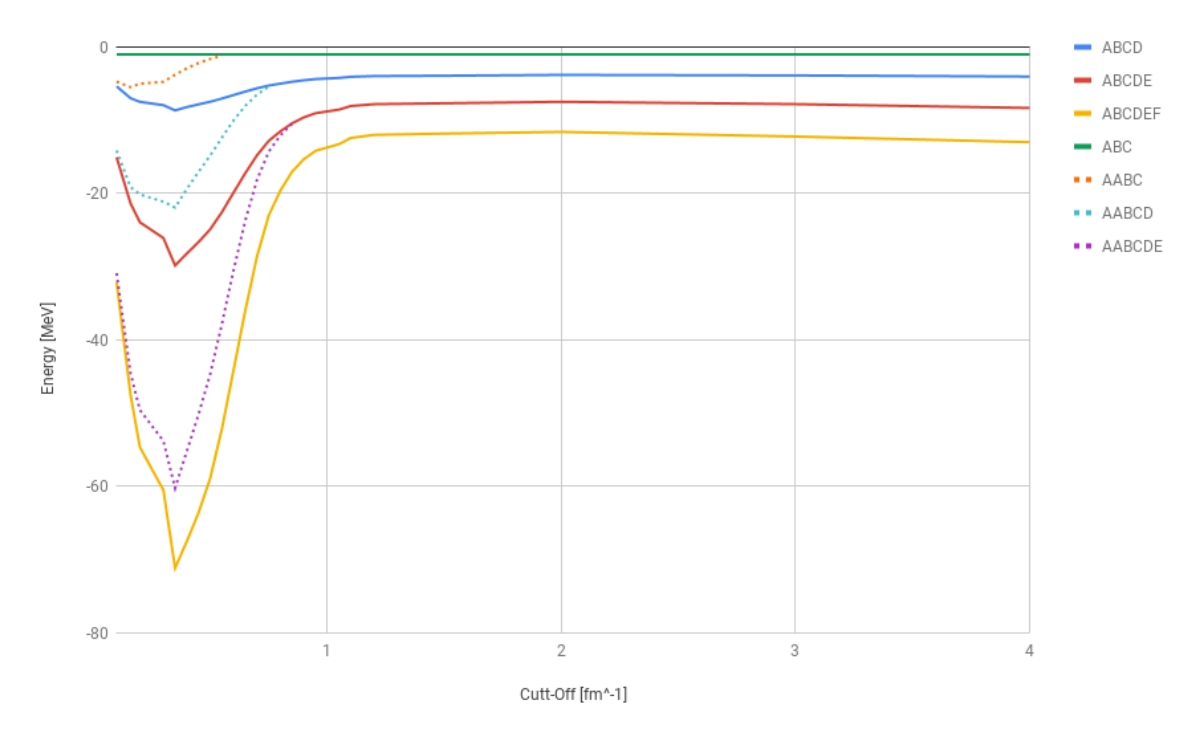
\includegraphics[width=\linewidth]{./unitarity_chart} 
        \caption{Cutoff dependence of ground-state energies of $A$-boson (solid line) and \abb (dashed line) systems 
        close the the unitary limit at which the dimer binding energy is at threshold $B(2)\to 0$,  and the trimer
        is kept at $B(3)=4$~MeV.}  
        \label{fig:unitary}
    \end{subfigure}
\caption{}
\end{figure} 

\subsection{Bosonic $1^{A}$ systems}
The $A$-boson ground states of a theory characterized by a Hamiltonian of
type \eqref{eq:hamiltonian}
has been numerically analysed in detail (see \eg~Refs.\cite{Bazak:2016wxm,2015PhRvA..92c3626Y,Gattobigio:2012tk,vonStecher:2011zz,Gattobigio:2011ey}).
In contrast to these studies, the bosonic interaction of this work supports
exactly one bound dimer and one trimer. The universal accumulation of trimers
at the $1+1$ body threshold is not considered. Furthermore, for all $\Lambda^*$
considered, only one $(A+1)$-boson state is found below
the $A$-boson threshold and no second as established numerically, \eg, in Refs.~
\cite{Hammer:2006ct,2009NatPh...5..417V,vonStecher:2011zz}.
Comparing the $A<7$ body spectra of $\Lambda^*=4$ with $\Lambda^*=3$ in
\figref{fig:threshold}, $B(A)/B(3)$ reduces, too. This indicates, that these states
resemble the shallow components of the conjectured universal pair. This hypothesis is
based on the argument that $\Lambda^*\to0$ is realized with an increasingly repulsive
three-body interaction which precludes the emergence of further $A$-boson bound states
but has an enhanced effect in a larger system as the number of triplets grows
with $A$. Therefore, one na\"ively expects a more rapid decrease of $B(A)$ \wrt $B(A-1)$ which compensates the initially found wider gap. To parametrize the
number $A^*$ at which $B(A^*+1)<B(A^*)$, \ie, stable $(A^*+1)$-body
cluster cease to exist, remains an open question.
For this work, we assume that $A^*=2$, which
means that for moving the trimer bound state closer to the dimer-boson threshold
the larger systems remain stable but they accumulate at the trimer-$(A-3)$-boson
threshold. This accumulation resembles the set of shallow states of the
alleged universal pair.

These considerations which identify the observed $A$-body states as ground
states are useful to characterize their spatial structure. The variational
bases expand only states with $L_\text{total}=0$. Yet, spatial configurations with
mixed symmetry are, in principle, allowed. However, interaction matrix elements
of such mixed states, \eg, particles occupying different oscillator $S$-shells
\scalebox{0.8}{$\young(\es,\zs)$}, 
should be of higher energy than a totally symmetric state
\scalebox{0.8}{$\young(\es\es)$}. For the three and four-body states we verified
this conjecture numerically for three- and four-body systems. To that end, a
resonating-group calculation which, in addition to $L_\text{total}=0$, projected
all relative motions between the particles (in Jacobi coordinates) onto $L=0$ was
employed. The contribution of configurations to $L_\text{total}=0$ from
Jacobi motion with $L>0$ was found increasingly insignificant with $\Lambda\to\infty$.

To summarize, we found the ground state of up to 7 bosons bound with respect to the
$B(A-1)$ threshold and spatially totally symmetric.
The convergence rate of $B(A)$ and $\rms{A}$ (within the considered cutoff range
$\Lambda\in[0.1,14]\fm$) increases with $\Lambda^*$, \ie, closer to the 
two-body unitarity limit, the bosonic
ground states become less sensitive with respect to details of the two- and three-body 
interactions. The finite dimer binding energy is identified as a parameter which
controls the existence of the universal pair of $A$-boson states -- shallow and deep
\wrt a universal $(A-1)$-boson state. For the considered values of $B(2)$ and
$\Lambda^*$, we identify only one element of the universal pair.

\subsection{Fermionic $\abb$ systems}
Now add one particle with an identical mass and
flavour-equal\footnote{
The identity of two out of 3 and 7 particles was enforced on the SVM basis
states, while these internal states were made totally
antisymmetric for any $A$-boson system. For $2+1^1$ particles, \eg, the 
spin-up/down states of a neutron suffice,
while for $2+1^3$, the spin and isospin formalism can be invoked.}
to one of the constituents of the above $A$-boson systems.

In a na\"ive approach, we
commence with spatial variational-basis states constrained to
a total orbital angular momentum $L_\text{total}=0$, as above.
Consequently, our SVM implementation with the antisymmetric constraint
on a pair of particles yields $B(A+1)<0$, \ie, no bound states.
Although, this can be proven analytically\footnote{} for contact interactions,
finite interaction ranges, \ie, $\forall\Lambda<\infty$, especially for
$\Lambda\ll 1\fm$, such bound states cannot be ruled out, {\it a priori}
because: one, a state with $L_\text{total}=0$ has non-zero overlap with 
mixed-symmetry states (as they are enforced by the internal wave-function component), 
and two, the finite range allows for 
non-zero matrix elements of the interaction even if two particles reside 
in different orbitals.
However, the results demonstrate the smallness of such transitions
which are necessary for the binding for reasonable ranges.

If the spatial component of the variational basis is projected
onto $L_\text{total}=1$, the eigenvalue spectra of
the $A+1\in[3,7]$ particle systems do contain a negative value ($B(A+1)>B(A)$ and
$L_\text{total}=1$ is understood from here on unless noted otherwise)
for $\Lambda\approx0.1\fm$.
In prose, if the regularized interaction provides enough attraction beyond
a repulsive region in which an effective
angular momentum barrier drives the particles apart,
the system's ground state is bound.
In order to assess the universal character of such a stable bound state
with mixed symmetry -- in other words, is $B(A+1)$ correlated
with $B(2,3)$ (neither of which is $f(\Lambda)$ by construction)? --
the cutoff is varied: $\Lambda\in[0.1,14]\fm$.

With increasing cutoff, \ie, decreasing interaction range, \ie, approaching the 
contact limit, $B(A+1)$ is found to decrease
and vanish for some critical value $\lc$. This critical
range increases linearly with $A$ (see \figref{fig:RGM1}).
The more particles in the bosonic ground-state core, the shorter-ranged the 
microscopic two- and three-body interaction
has to be in order not to stabilize the $A+1$ mixed-symmetry state.
As $\lc(A=2-6)$ are arguably small relative to a scale above
which the nuclear contact theory (\eftnopi) would
be useful, the result implies:

The absence of $L=1$, $S=1/2$, $A+1$-body bound states in an $A$-flavour theory
is a consequence of flavour-independent contact interactions which are
renormalized to one bound dimer and one bound trimer. 

Strictly speaking, the results presented thus far support this conclusion about the
universal instability of the $A+1$
body state only for $A=2-6$. In order to gain insight whether the linear
dependence of the critical range holds for
$A>6$, we employ a single-channel, effective two-fragments resonating-group
approximation (see \eg~Refs.~\cite{PhysRev.52.1083,Naidon_2016}). This approximation
turns the $A+1$ body problem into a two-body problem between a ``frozen'' 
core and one of the original particles of
the few-body problem. What makes this seemingly drastic simplification 
appropriate is the halo character of the problem,
namely, the increasingly large gap
$\lim_{\Lambda\to\infty}\left[B(A)-B(A-1)\right]=\infty$, which does not
allow for excitations of the bosonic core induced by the $A+1$-th particle if the
energy of the latter
does not exceed the scale set by this gap. It is helpful to consider this
treatment as a generalization of the
time-honoured description of the 5-nucleon system around the Nucleon-$\alpha$
threshold (see \eg~Refs.\cite{Bertulani:2002sz,Brown:2013zla} for the EFT formulation).

However, the RGM method does not model the core as point-like but retains
its finite size. It assumes
an independent motion of the core particles but takes into account (anti)
symmetrization.
The independent motion allows for a representation of the core by
its $A$-body ground state as it exists in the absence of the $A+1$-th particle.
As this state was shown
to be spherically symmetric with $L_\text{total}=0$, we choose to retain only one
component of an harmonic-oscillator (HO)
Slater-determinant expansion, \ie, a product of four single-particle HO
ground-state orbitals.
The $A+1$-body Schr\"odinger equation reduces to its two-body form by disregarding
variations of this wave function
while minimizing the corresponding functional only \wrt the component
which describes the relative motion.
In this course, the effect of the antisymmetrization between two of
the particles has to be considered and is reflected
in isolated components of the effective two-body potential.

We detail the parametrization of these various components of the core-particle 
interaction with the
microscopic coupling strengths $C_0$, $D_0$, the single-particle mass $m$, and the
 regulator parameter $\Lambda$
in an appendix~\ref{app:rgm}.
There, we split the effective potential in the customary three terms:
The direct potential, which averages the interaction of the orbiter with the core 
particles. This interaction is
local and resembles the character of the two-particle interaction for the 
fragment-relative coordinate. It does not
consider the statistical properties of the particles.
These properties lead to the non-local exchange interaction which contains an
 energy-dependent part which
is conventionally called the exchange kernel.

First, we shall discuss the case which disregards the exchange of the orbiter with 
one of the core constituents (local approximation).
The increase of the critical Gaussian cutoff $\lc$ with the number of
particles which we found by explicit $A$-body SVM calculations for $A<8$
continues in the RGM extrapolation up to a maximum number $\lc(A^*)$.
Both, $A^*$ and the associated $\lc(A^*)$ increase with $\Lambda^*$
(compare maxima of the three curves in \figref{fig:RGM2}).
The significance of this finding depends on the magnitude of $\lc$
relative the the breakdown scale ($\largescale$) -- any 
$\Lambda\lesssim\largescale$ affects the interaction at a range where
universal states are known
to reside for $\Lambda\to\infty$ but would surely ``feel'' the small-$\Lambda$
changes -- of the employed theory. For point particles, we estimate
$\largescale\approx m^{-1}=\mathcal{O}(10^{-1}\fm)$.
We find $\largescale<\lc$ for $A>3$ and conclude that the
stability of a fermionic system of point particles with mass $m$ and
finite $\Lambda^*$ depends on characteristics of the interaction which cannot
be observed in the bosonic ground states.
For particles whose substructure is known, \eg, nucleons as composites whose
excitations become relevant at energies of about the pion mass ($m_\pi$),
the above conclusion, namely 
\mbox{$\largescale\approx m_\pi^{-1}=\mathcal{O}(1\fm)<\lc$}
is satisfied for $A\gtrsim7$. The unbound character of five- and six-nucleons
are thus universal consequences of their particular two- and three-body subsystems.

To substantiate this conjecture, we fit the experimental deuteron and triton
binding energies, $B(2)=2.22$~MeV and $B(3)=8.48$~MeV, respectively. 
The spin singlet dibaryon (\eg, the dineutron) also bound with $B(2)$ as a consequence
of the assumed spin-independence of the leading-order theory.
The effect of a spin-dependent LO interaction which discriminates between a real
deuteron, and virtual singlets, has been found small (see \eg~Refs.\cite{Kirscher:2015yda,Konig:2016utl}), and in
particular, as the interaction in the other two-body channels is still
attractive -- the observed phenomena rest on the combinatorial enhancement of
attractive two- and three-body matrix elements (see appendix~\ref{app:rgm}) and
depend only in magnitude on those -- our qualitative results shall not change.

For $A\le 4$, we observe instability pattern qualitatively identical to
those shown in \figref{fig:threshold} for the corresponding $A+1$ systems.
Hence, the three-parameter theory predicts correctly the experimentally
established instability of nuclei in the
$^3p,\,^3n,\,^4\text{H},\,^4\text{Li},\,\text{and}~^5\text{He}$ channels.

In contrast, $^6$Li is known to sustain a $J^\pi=1^+ $ bound state
approximately $1.5~$MeV below the $\alpha$-deuteron threshold.
In order to make predictions with contact theories for this
three-proton and three-neutron ($2+2+1+1$) nucleus, the (iso)spin component of the SVM
wave function was chosen appropriately.
We find a particle-stable $^6$Li below a critical cutoff
$\lc\approx1.5\fm$, while for larger cutoffs,
\ie, a smaller interaction range, the ground state energy is
smaller than the sum of the consistently assessed deuteron and $\alpha$-particle binding
energies (see \figref{fig:nuclear}).
Analogously, we find $^8$Be ($2+2+2+2$) to become unstable \wrt an $\alpha$-decay at a
$\lc\approx 1\fm$, \ie, the same order as a nuclear interaction
range assumed to be mediated by pion exchange (see discussion above).
In contrast to the $\abb$ systems, $\lc$ decreases with the number of particles.

To understand this, we return to the one-particle-fragment motion relative to an $A$-particle core. 
For this motion being in an odd partial wave, repulsive components in
the effective -- direct and non-local exchange terms act analogous in the sense that the attractive
or repulsive character of one of their components is set solely by the respective two- or three-body
low-energy constant indicating its origin -- interaction resulting from an assumed\footnote{} repulsive
three-body contact are small compared with the attractive two-body terms for small $A$ and $\Lambda$.
Increasing any of the two parameters increases the repulsive three-body-related term, either because
the running of $\led$ exceeds $\Lambda^6$, eventually, or via a dominance of the triplets over
pairs in the many-body system.
While this dependence on $A$ and $\Lambda$ suggests that for larger $A$ the weakening of attractive along
an enhancement of the repulsive components of the potential also reduces $\lc$ the exponentially
increase in range of both through the implicit dependence of $a$ on $A$ is larger in case of the
attractive two-body remnant. The slower extension of its range, however, eventually is compensated by
the quadratic growth of the strength of the repulsive three-body parts (given reasonable assumptions, \eg, liquid drop,
about the $a(A)$ relation). 
This explains qualitatively the initial increase of $\lc$ with $A$ up to an $A^*$ (range dominance) beyond which
number, $\lc$ should decrease (as discussed in \figref{fig:RGM2}) in consequence of the quadratic strength
increase of the repulsive interaction component (combinatorial strength dominance).

In an even partial wave, the effective interaction strengths between the core and a single particle are reduced
by considering the exchange of the particle with one core element. In addition, the independent motion of the particles
during the exchange introduces and interaction-independent repulsion in an even partial wave (exchange kernel).
These two effect combined disfavour a stable state.

If, however, there is an even number of particles exchanged between the fragments (two in the case of $^6$Li, and
four for $^8$Be), the effective potential changes by additional terms pertaining to these elements of the
antisymmetrizer. Those new components introduce the opposite behaviour, namely, an enhancement of a coupling strength
in an even partial wave and a mitigation in an odd one.

Even relative angular momentum, at low $\Lambda$, weakens the attractive $\lec$-proportional
and the repulsive $\led$-proportional term.
The component of the potential which supports binding is thereby reduced and the combinatorially-enhanced
balance relative to the repulsive three-body term is dominated by the latter already for smaller $A$.

The meaning of $\lc$, however, is unchanged.
Once the cutoff exceeds these critical values in the course of taking the
zero-range limit, neither $^6$Li nor $^8$Be are predicted particle stable
by the leading-order theory.

The implication of this result for the usefulness of the pionless leading-order effective field theory for
the description of these nuclei, the trajectory of the bound-state poles through the respective thresholds at $\lc$
is crucial.
To this end, we apply the method of analytical continuation in the coupling
constant (ACCC, see, \eg~Ref.~\cite{Kukulin_1977}) to the $2+1$ case which represents, \eg, a three-neutron system.
Thereby, an attractive three-body contact term is introduces with strength $d_0^\Lambda$ of the same structure as the one
which renormalizes the bosonic three-body system in \eqref{eq:hamiltonian}. The delta functions of this term use a
cutoff parameter $\Lambda$ which is identical to the two-body cutoff. For a range of cutoffs
(see \figref{fig:poletrajectory}), the initial $d_0^\Lambda$ was chosen to bind the $2+1$ system before taking
the limit $d_0^\Lambda\to 0$ while following the bound state pole on its way on the physical (energy) sheet through
the branch cut starting at $E=0$ from above onto the fourth quadrant of the unphysical sheet. On The latter (hatched
area in \figref{fig:poletrajectory}), it represents a resonance. The pole remains on this sheet for
$\Lambda\lesssim4\fm$. For larger cutoffs, the pole passes through another branch cut and leaves the first
unphysical sheet. Thus, it no longer represents a dimer-particle resonance. Furthermore, its trajectory does not
indicate to converge to a point on this second unphysical sheet. This behaviour suggests that an analogue of the dynamical
pole generated (not generated by a single diagram but rather an infinite geometric series) by the
contact theory \eqref{eq:hamiltonian} in the two- and three-boson systems, does not
exist in \abb, neither as a bound nor resonant state.

\begin{figure}[h] 
\centering 
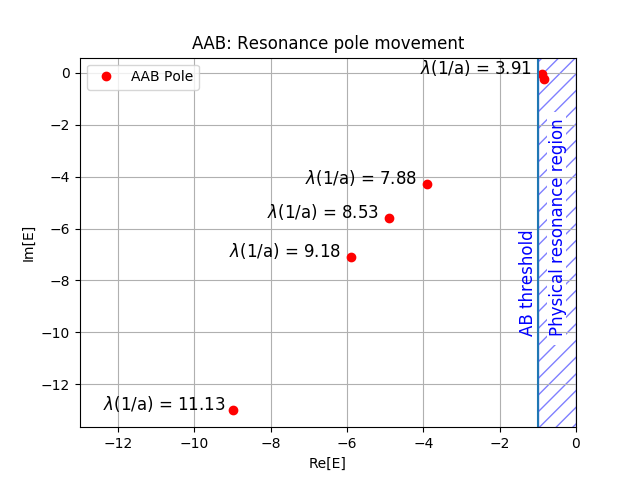
\includegraphics[width=0.8\textwidth]{./AAB_resonance_run.png} 
\caption{Lowest Hamiltonian eigenvalue analytically continued below the lowest
two-/three-fragment breakup (ordinate/vertical at Re$[E]=-1~$MeV) threshold
for a $2+1$ system. Eigenvalues in the hatched region correspond to resonances
which disappear with increasing regulator cutoff ($\lambda$ label) through the
three-fragment breakup branch cut.}
\label{fig:poletrajectory}
\end{figure}
%Studying the spectrum of the $A^2B^2CD$ system ($^6$Li if fitted on nuclear observable), 
%more than one state appear to be stable for very small $\Lambda$.
%All those states becomes unstable for large $\Lambda$. 
%Studying the order of the states and the order of disappearance (see \tabref{tab:levelorder}),
%it well represent the expected one for the physical $^6$Li despite the oversimplified interaction used.

To relate this observation to \eftnopi, in particular,
the magnitude of the critical cutoff relative the scales in the theory is of importance.
$\lc$ for $^6$Li is arguably of the same order as the breakdown scale $\lc\sim1.5$ fm$^{-1} \approx300$ MeV set by
the pion mass.
The EFT framework demands to study cutoff/renormalization-group independence of the theory at values
significantly larger than any presumed breakdown scale.
Thereby, the interpretation of the stable six-body bound states as a cutoff artefact is justified.

For the conception of an extension of the \eftnopi which predicts also the particle-stable character of
$^6$Li and $^8$Be in the zero-range limit, we analyse the mechanism behind the stability of these
systems for $\Lambda<\lc$. Of all artefacts introduced by the finite range of the regulated contact interaction,
we single out: First, a finite effective range in the two-body $S$-wave channel, and second, a non-zero, attractive
two-body $P$-wave interaction. Both contribute to the attraction in the \abb~system but their relative
significance in this role is obscure.
%\textbf{Projecting the interaction} discriminate between the contribution of different partial waves
% ( and different orders of the theory) included into the finite cut-off interaction.
%In facts, the Gaussian regulator expanded in partial waves contains any-order partial waves.
%Larger angular momentum contributions disappear only when the cut-off is increased,
% but are still relevant in the region in which P-wave states are stable. 
In other words, the finite-range interaction does not only describe a finite but large $S$-wave scattering length
but also other finite parameters of the effective-range expansion of the $S$-wave amplitude, the $S$-wave
effective range $r_0$ being one of these. Furthermore, the scattering volume $a_1$ of the two-nucleon $P$-wave amplitude is
non-zero.
%Both contributions are expected to enter only subleading in the system description but contribute to
%the stabilization of P-wave systems at low cut-off.
By studying the sensitivity of the bound \abb system below \lc~\wrt a variation of either of those
parameters instead of the combined change as induced by varying $\Lambda$ as in the analysis presented thus far,
insight about the order of a potential enhancement of the corresponding higher-order-in-LO-\eftnopi vertices 
is gained.

First, we project the two-body interaction in a spin 0, \ie, an asymmetric internal state.
This forces two interacting particles into an even spatial state. Non-zero matrix elements between states
in odd partial waves cancel.
The effect of removing this contribution is shown in \figref{fig:Sprojection}. Namely, a significant
reduction of $\lc^A$. 
Without the residual attraction in odd partial waves, the binding is attributed mainly to the finite $r_0$ and
a coupling to even larger relative two-body angular momenta.

\red{What is our proposal for a contact theory which describes all what \eftnopi~does and 6Li et al.?}



%Defining an effective theory as in equation \ref{eq:hamiltonian}
% with $C_0$ and $D_0$ fitted to reproduce the two- and 
%three-body energies defined in \tabref{tab:configurations}, the energy of
% varius P-wave systems are calculated.
%Using SVM the ground state energies of up to $A+1=$ 7 isomassive fermions with 
%$A \le $6 flavors are calculated.
%The same is done up to $A+1\sim$60 $A$-flavour fermionic systems using resonating 
%group method (RGM).
%In the case of $A$ \textit{different} fermions the ground state is spatially symmetric.
%No spin dependence is included in our model, therefore, those systems behaves as if 
%composed of bosons (it is boson-like) 
%and are equivalent to the case discussed in \cite{manybosons}.
%Convergence of the ground state energy of bosonic-like system with respect to the 
%cut-off is observed for all the theory 
%input used in this work.
%We observe and increasing of the ground state binding with the number of particles. 
%The point radius $\langle r^2 \rangle$ has been calculated for $A\le6$, for a number 
%of systems too small to extrapolate the 
%behavior for large $A$, however, we expect it to behave as $A^{1/3}$ as predicted by 
%the neutron drop model and observed in  
%\cite{manybosons}.
%
%Adding an extra fermion with the same flavor as one in core to the system,
%we observe the groundstate wavefunction to be 
%spatially asymmetric, and with angular momentum L=1.
%However, this state remains stable only for small cut-off after which the systems 
%breaks in the symmetric core and the extra 
%fermion.
%This is a common behaviour of all the systems and input configurations considered.
%In \figref{fig:treshold}, are compared the ground-state energy of the $A\le 6$
%bosonic-like fermionic system and the 
%L=1 $A$+1 bindings for $B(3)=3$ and $4$ MeV.
%For each number of particles a critical cut-off $\lc^A$, corresponding to the 
%cut-off in which the $A+1$ state becomes 
%unstable, exists.
%For larger cut-offs, the ground-state energy coincide with the one of the $A-$fermion 
%systems and the system breaks in a $A-$
%particles symmetric subsystem and a free fermion.
%The result for $A^2B$ fermions is in agreement with the one found by Kartavtsev et al. 
%\cite{Kartavtsev_2007} in the 
%particular case in which the fermions are isomassive.

\begin{figure}
\centering
\begin{subfigure}[t]{0.49\textwidth}
\centering
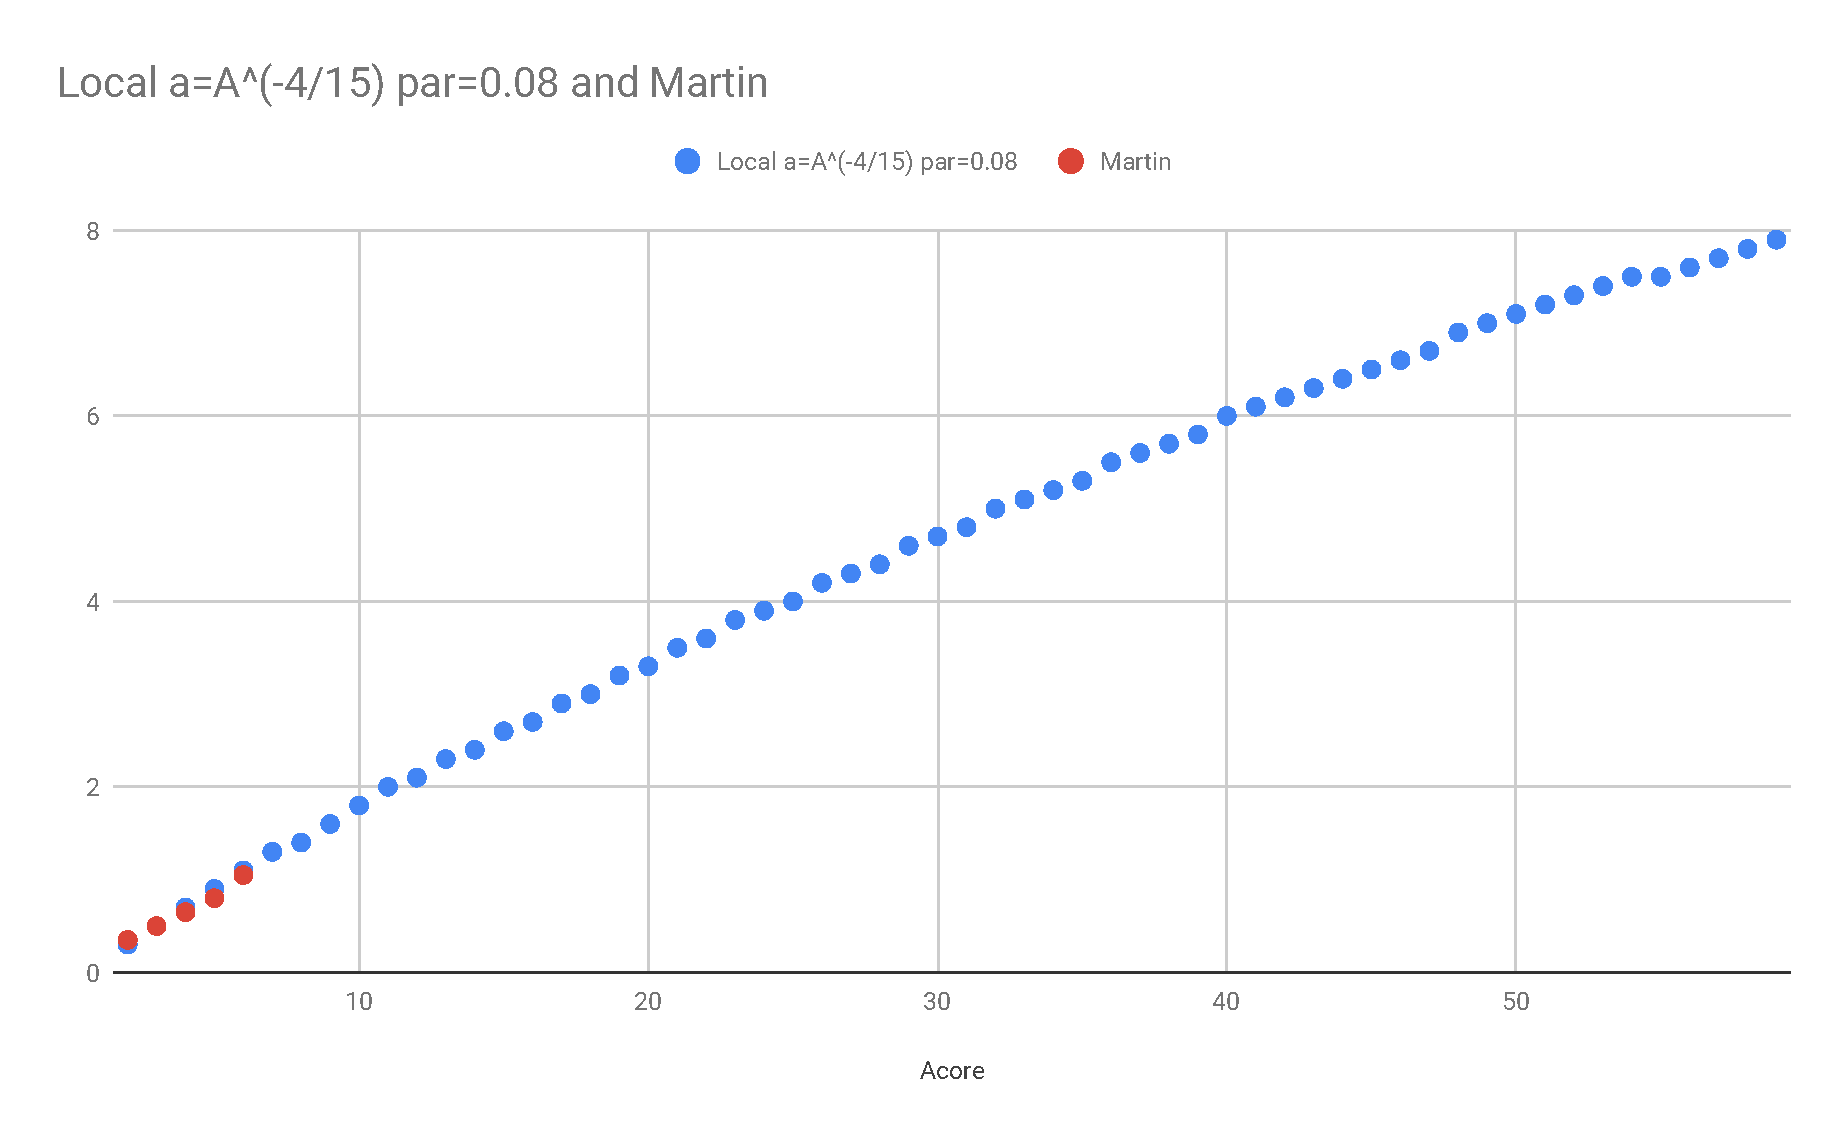
\includegraphics[width=0.9\textwidth]{./local2}
\caption{}
\label{fig:RGM1}
\end{subfigure}
    \hfill
\begin{subfigure}[t]{0.49\textwidth}
\centering
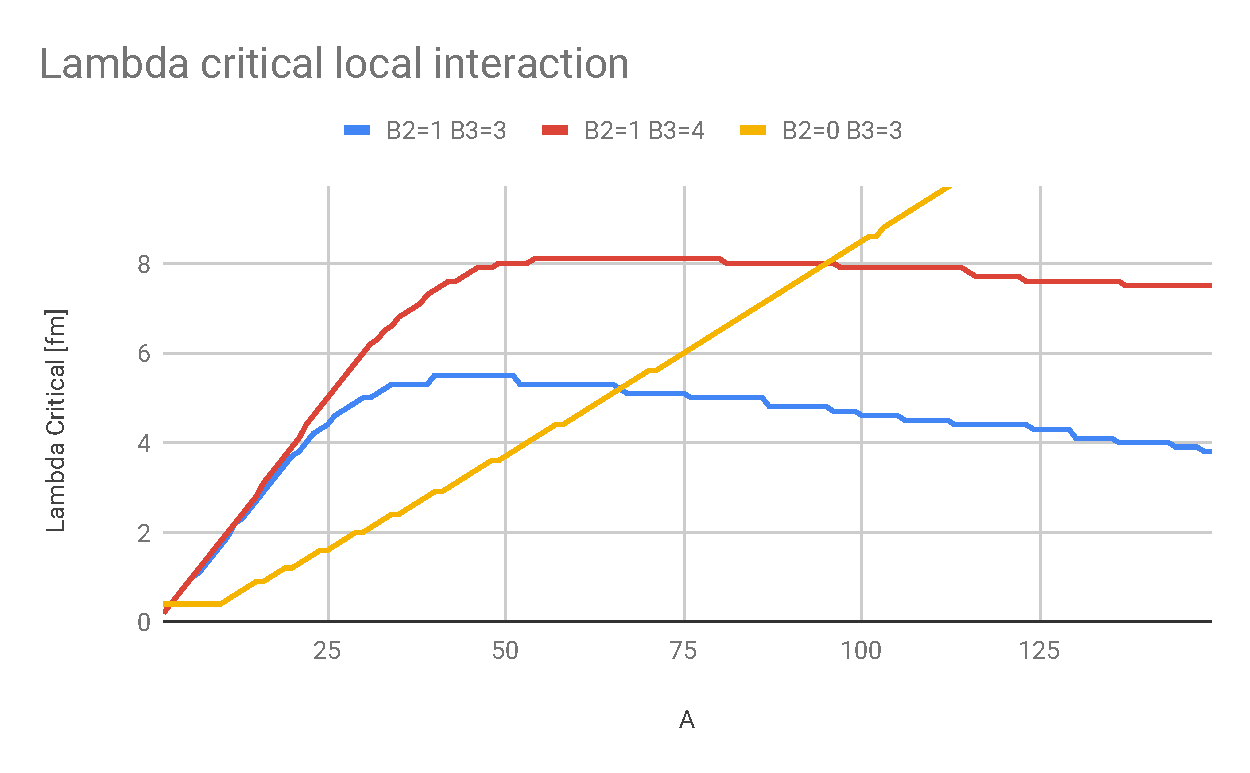
\includegraphics[width=0.9\textwidth]{./local_large} 
\caption{}        
\label{fig:RGM2}
\end{subfigure}
\caption{Dependence of the critical cutoff ($\lc$) on the number of core particles ($A$).
Red dots in (a) mark SVM few-body calculations.
All other curves represent results obtained within a single-channel resonating-group method.
In (b), the effect of a change in the ratio between two- and three-boson binding energies on $\lc$ is shown.
For $B(2)=0$, the respective scattering length $\to\infty$.}
\label{fig:RGM}
\end{figure}

%\textbf{Larger systems} 
%are not accessible with ab-initio few-body methods like SVM. 
%For this purpose an extension of resonating group 
%method (RGM) \cite{PhysRev.52.1083,Naidon_2016} has been developed.
%From the fundamental two- and three-body interaction, a potential between the
% spatially symmetric core and the remaining fermion is extracted. 
%In principle this permits to reduce a complex many-body calculation in a simpler 
%two-body problem at the price of having non-local and energy dependent interaction.
%The derivation is done assuming that the wave function of the core is frozen to be the
% harmonic oscillator (HO) Hartree Fock (HF) ground state with respect to the system 
% center of mass.
%The oscillator parameter is fixed to reproduce the HO ground state point radius 
%$\sqrt{\langle r^2 \rangle} \propto A^{1/3}$.
%$\alpha$ is fitted to reproduce the $\lc^{3\le A \le 6}$ from SVM calculations.
%In \figref{fig:RGM} is shown the behavior for $A \le 60$ using RGM with local 
%approximation for different configuration of the theory. 
%We observe an increasing of $\lc^A$ with $A$, remaining finite for all the 
%systems considered.
%In one hand, this means that adding more particles in the spatially symmetric core of 
%the system, the P-wave states becomes more stable and for any $r_0$ there is a minimal 
%$A$ after which it stabilize (see equation \ref{eq:philips_effr} for 
%$\Lambda\leftrightarrow r_0$ correspondence).
%On the other one, there is always a $\lc^A$ for which the P-wave state becomes 
%unstable and in the contact limit all P-wave systems decay in the symmetric core and 
%one particle.
%Comparing  $\lc^A$  with the scale of the system (the mass of the particles), it 
%results that the unstability always happens far from the expected renormalization 
%invariant reagion.
%This remains true also when we consider nuclear mesonic scales.
%In facts, introducing a new breaking scale $M_{hi}\sim M_{\pi}\approx 140$ MeV we 
%expect to reach renormalization invariance for $\Lambda\ll M_{\pi} a \sim 10-40$ which 
%is larger or comparable with the critical cut-off we observe.
%
%--- This behavior can be seen for different configuration of two and three body 
%bindings close to universality.
%Studying $\lc^A$ behavior with the non-universal parameter $B(3)/B(2)$ ... need 
%more data here to do the comparison. ---


\begin{figure}[h] 
\centering 
\begin{floatrow}
\ffigbox{
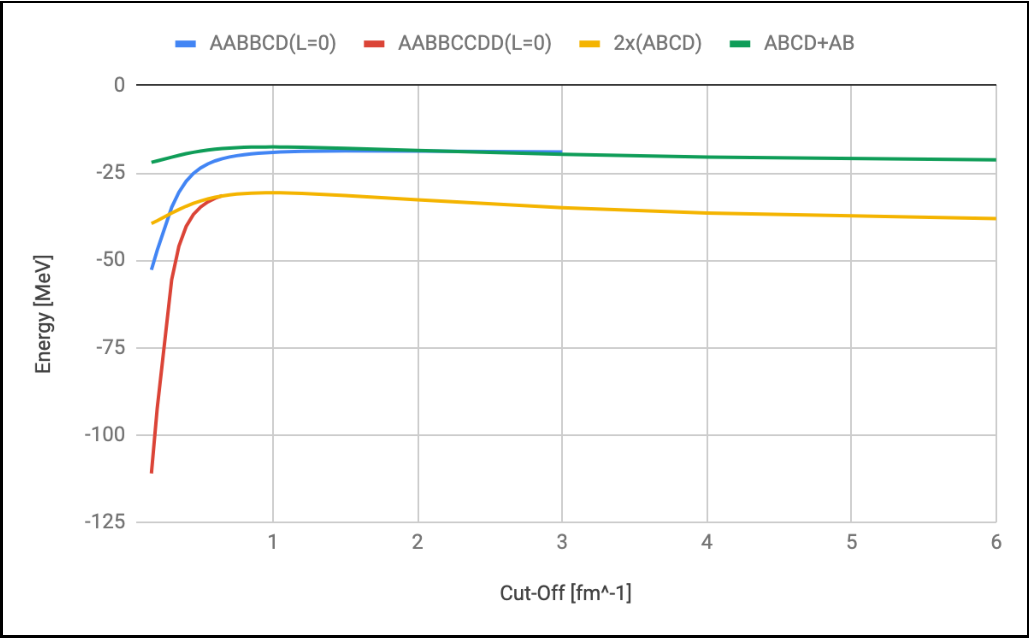
\includegraphics[width=0.45\textwidth]{./Nuclear} 
}{
\caption{Cutoff dependence of the lowest Hamiltonian eigenvalue in the $^8$Be (red) and $^6$Li (blue) channels along with 
the lowest threshold, $\alpha$-$\alpha$ (yellow) and $\alpha$-deuteron (green), respectively.
%The instability of P-wave system is observed also if the theory is fitted to reproduce nuclear two- and three-body bindings.
}
\label{fig:nuclear}
}

\capbtabbox{%
\centering 
\begin{tabular}{ccc}
System & $2+2$ & $2+2+1+1$ \\\hline\hline
$L_{\text{\scriptsize total}}$ & $r_c$ [fm]& $r_c$ [fm]\\
0 & 4.16 & 1.23 \\
1 & 5.21 & 2.96 \\
2 & 4.81 & 2.30 \\
\end{tabular}
}{\caption{Minimal effective range to stabilize the $2+2$ (dimer-dimer)
and the $2+2+1+1$ ($^6$Li nucleus) systems in different partial waves.
%Despite the simple interaction the level order well represent the one observed
%for $^6Li$ \cite{Chadwick20112887}. Nonetheless, for small effective range
%(large cut-off) all these states become unstable. 
}\label{tab:levelorder}}
\end{floatrow}
\end{figure} 


\begin{figure}[h] 
\centering 
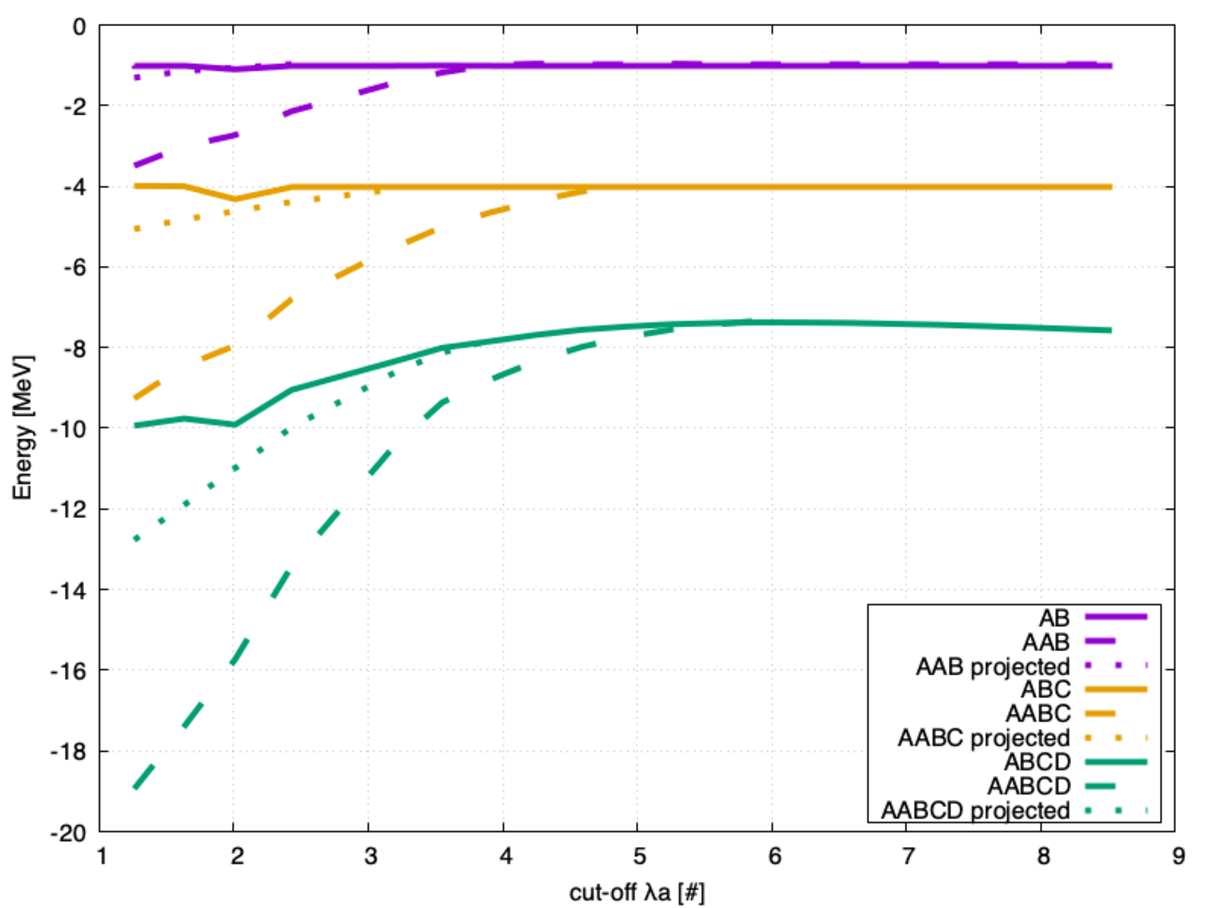
\includegraphics[width=0.8\textwidth]{./Sprojection} 
\caption{Cutoff dependence of the lowest energy eigenvalue of an \abb~fermionic systems ($A=2$: purple, $A=3$: beige, $A=4$: green) as predicted with a
projected (dotted line) and non-projected (dashed lines) interaction along with the lowest threshold set by
the ground-state energy of the spatially symmetric $A$-boson core.}
\label{fig:Sprojection}
\end{figure} 

\section{Conclusion}
A non-relativistic system of $A+1$ particles with identical masses and
an $A$-dimensional internal flavour space cannot sustain a bound state if
its dynamics is constrained by representations of two- and three-particle
momentum-independent contact interactions which are renormalized to yield
a bound/unitary two-body state and a bound three-body state and whose
residual finite-range is below a critical value ($\lc^{−1}$)
which decreases with increasing particle content $A$ of the system.
If the range of the regulated contact interactions, however, surpasses the
critical range, the ground state of the $A+1$ particles is bound with respect
to breakup in the bosonic, spatially symmetric $A$-body ground state and a
single free particle. The total orbital angular momentum of this $A+1$ bound
state is $L_{\text{\scriptsize total}}= 1$.
For any finite ratio $\Lambda^*<\infty$,
the critical range reaches a minimum at a certain number of particles $A$.

\section{Appendix: Inter-cluster Potential}\la{app:rgm}
We shall sketch the derivation of the potential between a core system of $A$ equal-mass bosons (spatially symmetric
in a ground state with energy $B(A)$) and a single particle (mass-equal to all but flavour identical to only one
of the core constituents) as it follows from a two- and three-boson contact interaction as discussed above following
\eqref{eq:hamiltonian}. Such an effective 2-body potential is appropriate for the description of the $A+1$ body amplitude
close\footnote{The energy of the relative motion is small relative to the splitting between $B(A)$ and the
next-lowest $A$-body threshold} to the $A+1$ normal threshold. We assume that the wave functions of stable \abb~structures
which were found in the explicit $A+1$ body calculations either below $\lc$ or via the ACCC procedure at this
$Am$ branch point are dominated by a two-fragment configuration of an inert core and a single particle. This
assumption is equivalent to the single-channel version of a resonating-group formulation of the many-body problem
(see \eg~Ref.\cite{TANG1978167}) and reduces the $A+1$ body Schr\"odinger equation to

\be\la{eq:rgm}
\bra\phi_A\hl\big(\hat{T}_{\ve{R}}+\hat{V}_\text{\tiny A,A+1}-E\big)\hat{A}\left[\phi_A\psi(\ve{R})\right]\ket=0\;\;,
\ee 

which is an equation for the relative motion $\psi$ (a function of the relative distance between the centre of mass
between the core and the particle's location) between the core in state $\phi_A$ and a single particle.
The average is taken \wrt the internal coordinates\footnote{We chose coordinates relative to the centre of mass of
the fragment, \mbox{$\vcl{i}:=\vsp{i}-\frac{\scriptstyle \sum_{i=1}^A\vsp{i}}{A}\;\;\;i\in\lbrace 1,\ldots,A\rbrace$},
and assume without loss of generality that particles $A$ and $A+1$ are identical.}
of the fragment \mbox{$\bra\ldots\ket=\prod\limits_{i=1}^{A-1}\int d^3\vcl{i}$}, \mbox{$E=E_\text{total}-B(A)$},
\mbox{$\hat{A}=\mathbb{1}-\hat{P}(\vsp{A}\leftrightarrow\vsp{A+1})$}, and
\begin{gather}
\hat{V}_\text{\tiny A,A+1}=~\lec\sum\limits_{i\leq A}\delta_\Lambda(\vsp{i}-\vsp{A+1})\nonumber\\
~+D_1^\Lambda\sum\limits_{i\neq j\atop \leq A}\left\lbrace\delta_\Lambda(\vsp{i}-\vsp{A+1})\delta_\Lambda(\vsp{j}-\vsp{A+1})
+\delta_\Lambda(\vsp{i}-\vsp{A+1})\delta_\Lambda(\vsp{j}-\vsp{j})\right\rbrace\;\;.
\end{gather}

We approximate the ground-state core wave function with

\be\la{eq:corewf}
\phi_A:=e^{-\frac{a}{2}\sum_{i=1}^{A}\vcl{i}^2}\;\;,
\ee

which is a localized, totally symmetric state parametrized by an
oscillator strength of unknown dependence on $A$ and $\Lambda$. The average over internal coordinates
can then be evaluated analytically, and the resultant equation projected into partial waves
assumes the final, non-local form

\begin{subequations}\la{eq.rgm.pw}
\begin{gather}
\int\Bigg\lbrace\frac{\hbar^2}{2\mu}\left[-\partial^2_R\left(\mathbb{1}+(\mathfrak{o}_E\leftrightarrow\mathfrak{o}_\mu)\right)+
\frac{l(l+1)}{R^2}\left(\mathbb{1}+(\mathfrak{o}_E\leftrightarrow\mathfrak{o}_L)\right)\right]
\phi_{lm}(R\mprime)\la{eq.rgm.pw.a}\\
%
-E\left(\delta(R-R\mprime)+(-)^{l+1}\mathfrak{o}_E(1)\left(\frac{a}{\pi}\right)^{3/2}
e^{+\frac{1}{2}\mathfrak{o}_E(aA^{-1})RR\mprime-\frac{1}{2}\mathfrak{o}_E(a)\ve{R}^2-\frac{1}{2}\mathfrak{o}_E(a)\ve{R}'^2}\right)\la{eq.rgm.pw.b}\\
%
+\mathfrak{o}_2(A)\cdot\frac{\lec}{\Lambda^3}\cdot a^{\frac{3}{2}}\cdot
e^{-\mathfrak{o}_2(a)\ve{R}^2}
\left(\delta(R-R\mprime)+(-)^{l+1}\mathfrak{o}_2(1)\left(\frac{a}{\pi}\right)^{3/2}
e^{+\mathfrak{o}_2(aA^{-1})RR\mprime-\mathfrak{o}_2(a)\ve{R}'^2}\right)\la{eq.rgm.pw.c}\\
%
+2\cdot\mathfrak{o}_3(A^2)\cdot\frac{\led}{\Lambda^6}\cdot a^{3}\cdot
e^{-2\mathfrak{o}_3(a)\ve{R}^2}
\left(\delta(R-R\mprime)+(-)^{l+1}\mathfrak{o}_3(1)\left(\frac{a}{\pi}\right)^{3/2}
e^{+2\mathfrak{o}_3(aA^{-1})RR\mprime-2\mathfrak{o}_3(a)\ve{R}'^2}\right)
\Bigg\rbrace\phi_{lm}(R\mprime)dR\mprime\la{eq.rgm.pw.d}\\
 =0\;\;\;.\nonumber
\end{gather}
\end{subequations}

The quantities $\mathfrak{o}_x$ represent numbers of order one times the arguments in braces.

\newpage
\section*{References}
\bibliographystyle{ieeetr}
\bibliography{Thebibliography.bib}
\end{document}
